\section{Mixed FE--meshfree formulation with optimal constraint ratio}

In the proposed mixed--formulation, the displacement is approximated using 3--node (Tri3), 6--node (Tri6) triangular elements and 4--node (Quad4), 8-node (Quad8) quadrilateral elements in 2D, 4--node (Tet4) tetrahedral element and 8--node (Hex8) hexahedral element in 3D \cite{hughes2000}. In order to flexibly adjust to let the DOFs of pressure meet the optimal constraint, the reproducing kernel meshfree approximation is involved to approximate pressure.

\subsection{Reproducing kernel meshfree approximation}

In accordance with the reproducing kernel approximation, the entire domain $\Omega$, as shown in Figure \ref{fg:rk_approximation}, is discretized by $n_p$ meshfree nodes, $\{\boldsymbol{x}_I\}_{I=1}^{n_p}$. The approximated pressure, namely $p_h$, can be expressed by the shape function $\Psi_I$ and nodal coefficient $p_I$, yields:
\begin{equation}
p_h(\boldsymbol{x}) = \sum_{I=1}^{n_p} \Psi_I(\boldsymbol{x}) p_I
\end{equation}
where, in the reproducing kernel approximation framework, the shape function $\Psi_I$ is given by:
\begin{equation}\label{rkshape}
\Psi_I(\boldsymbol{x}) = \boldsymbol{c}(\boldsymbol{x}_I-\boldsymbol{x}) \boldsymbol{p}(\boldsymbol{x}_I-\boldsymbol{x}) \phi(\boldsymbol{x}_I - \boldsymbol{x})
\end{equation}
in which $\boldsymbol{p}$ is the basis vector, for instance in the context of the 3D quadratic case, the basis vector takes the following form:
\begin{equation}
\boldsymbol{p}(\boldsymbol{x}) = \{ 1, x, y, z, x^2, y^2, z^2, xy, xz, yz\}^T
\end{equation}
and $\phi$ stands for the kernel function. In this work, the traditional Cubic B--spline function with square or cube support is used as the kernel function:
\begin{equation}
\phi(\boldsymbol{x}_I-\boldsymbol{x}) = \phi(s_x) \phi(s_y) \phi(s_z), \quad s_i = \frac{\|\boldsymbol{x}_I - \boldsymbol{x}\|}{\bar{s}_{iI}}
\end{equation}
with
\begin{equation}
\phi(s) = \frac{1}{3!} \begin{cases}
(2-2s)^3 - 4(1-2s)^3 & s\le\frac{1}{2} \\
(2-2s)^3 &\frac{1}{2}<s<1 \\
0 & s> 1
\end{cases}
\end{equation}
where $\bar{s}_{iI}$'s are the support size towards the $i$-direction for the shape function $\Psi_I$. The correction function $\boldsymbol{c}$ can be determined by the following so-called consistency condition:
\begin{equation}\label{cc1}
\sum_{I=1}^{n_p} \Psi_I(\boldsymbol{x}) \boldsymbol{p}(\boldsymbol{x}_I) = \boldsymbol{p} (\boldsymbol{x})
\end{equation}
or equivalent shifted form:
\begin{equation}\label{cc2}
\sum_{I=1}^{n_p} \Psi_I(\boldsymbol{x}) \boldsymbol{p}(\boldsymbol{x}_I-\boldsymbol{x}) = \boldsymbol{p} (\boldsymbol{0})
\end{equation}
The consistency condition ensures that the reproducing kernel shape functions are able to reproduce the polynomial space spanned by the basis function $\boldsymbol{p}$, which is a fundamental requirement for the accuracy of the Galerkin method.
Herein, the order of the basis function $\boldsymbol{p}$ is chosen to be the same as the order of the displacement approximation.

Further, substituting Eq. \ref{rkshape} into Eq. \eqref{cc2} leads to:
\begin{equation}\label{correction}
\boldsymbol{c}(\boldsymbol{x}_I-\boldsymbol{x}) = \boldsymbol{A}^{-1}(\boldsymbol{x}_I-\boldsymbol{x}) \boldsymbol{p}(\boldsymbol{0})
\end{equation}
in which $\boldsymbol{A}$ is namely the moment matrix evaluated by:
\begin{equation}
\boldsymbol{A}(\boldsymbol{x}_I-\boldsymbol{x}) = \sum_{I=1}^{n_p} \boldsymbol{p}(\boldsymbol{x}_I-\boldsymbol{x}) \boldsymbol{p}^T(\boldsymbol{x}_I-\boldsymbol{x}) \phi(\boldsymbol{x}_I-\boldsymbol{x})
\end{equation}
Taking Eq. \eqref{correction} back to Eq. \eqref{rkshape}, the final form of the reproducing kernel shape function can be obtained as:
\begin{equation}
\Psi_I(\boldsymbol{x}) = \boldsymbol{p}^T(\boldsymbol{0}) \boldsymbol{A}^{-1}(\boldsymbol{x}_I-\boldsymbol{x}) \phi(\boldsymbol{x}_I-\boldsymbol{x})
\end{equation}

As shown in Figure \ref{fg:rk_approximation},
reproducing kernel meshfree shape functions are globally smooth across the entire domain,
using them to discretize the pressure field allows the constraint ratio to be adjusted arbitrarily, without being limited by element topology.
Meshfree shape functions generally lack the Kronecker delta property, which prevents the direct imposition of essential boundary conditions.
Fortunately, the mixed formulation shown in Eq. \ref{ritz_Galerkin} only concerns the displacement essential boundary condition, and this condition can be easily imposed by the standard methods, such as the penalty method that used in this work.

Moreover,
when combined with finite element approximations in Eq. \ref{ritz_Galerkin},
numerical integration can be conveniently performed within each finite element ($\Omega_C$'s).
The numerical integration issue caused by the loss of variational consistency between meshfree shape functions and their derivatives \cite{wu2021} would not appear in the mixed formulation of Eq. \ref{ritz_Galerkin}, this is due to the fact that Eq. \ref{ritz_Galerkin} solely depends on the meshfree shape functions themselves.
Therefore, the proposed method employs standard lower-order Gaussian quadrature rules, as commonly used in traditional finite element methods, while still maintaining its accuracy.

\begin{figure}[H]
\centering
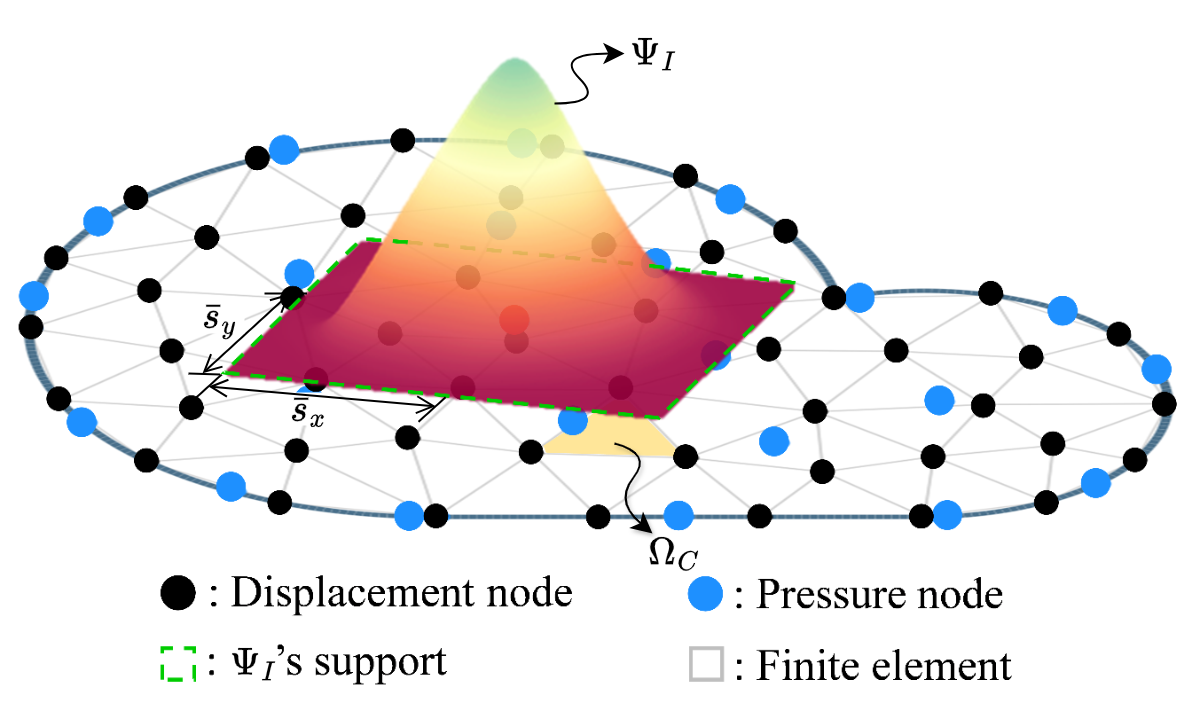
\includegraphics[width=\textwidth]{png/mix.png}
\caption{Illustration for reproducing kernel meshfree approximation}\label{fg:rk_approximation}
\end{figure}

\subsection{Pressure node distributions with optimal constraint ratio}\label{subsec:optimal_constraint_ratio}

In this subsection, 2D and 3D inf-sup tests \cite{chapelle1993}, as defined in Eq. \ref{infsup_test}, are conducted using the mixed FE-meshfree formulations to validate the proposed inf-sup value estimator.
The 2D test considers the square domain $\Omega = (0,1)\times (0,1)$, where the displacement is discretized by Tri3 and Quad4 with $4\times 4$, $8\times 8$, $16\times 16$ and $32\times 32$ elements, Tri6 and Quad8 with $2\times 2$, $4\times 4$, $8\times 8$ and $16\times 16$ elements, respectively. The 3D test employs a cube domain $\Omega = (0,1)\times (0,1)\times (0,1)$ with $4\times 4$, $8\times 8$ and $16\times 16$ elements for the Tet4 and Hex8.
For pressure discretization, linear meshfree approximation with a normalized support size of $1.5$ is employed for Tri3, Quad4, Tet4 and Hex8.
For Tri6 and Quad8, a quadratic meshfree approximation with a normalized support size of $2.5$ is utilized.
In order to avoid the influence of interpolation error, uniform nodal distributions are used for pressure discretizations, for example in Figure \ref{fg:infsup_mesh}, which displays $4\times4$ Quad4 elements with $4\times3$ uniformly distributed pressure nodes.

\begin{figure}[H]
\centering
% 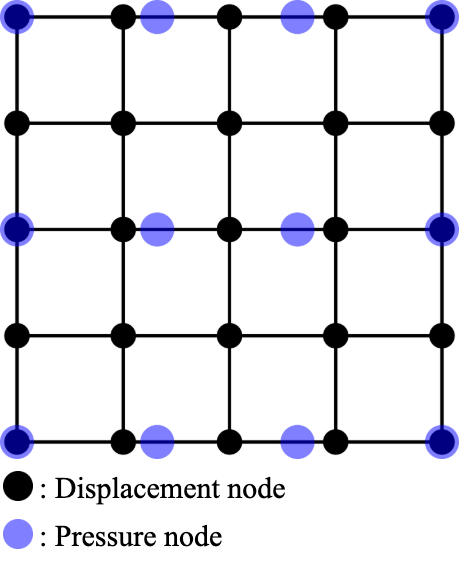
\includegraphics[width=0.5\textwidth]{png/infsup_mesh.png}
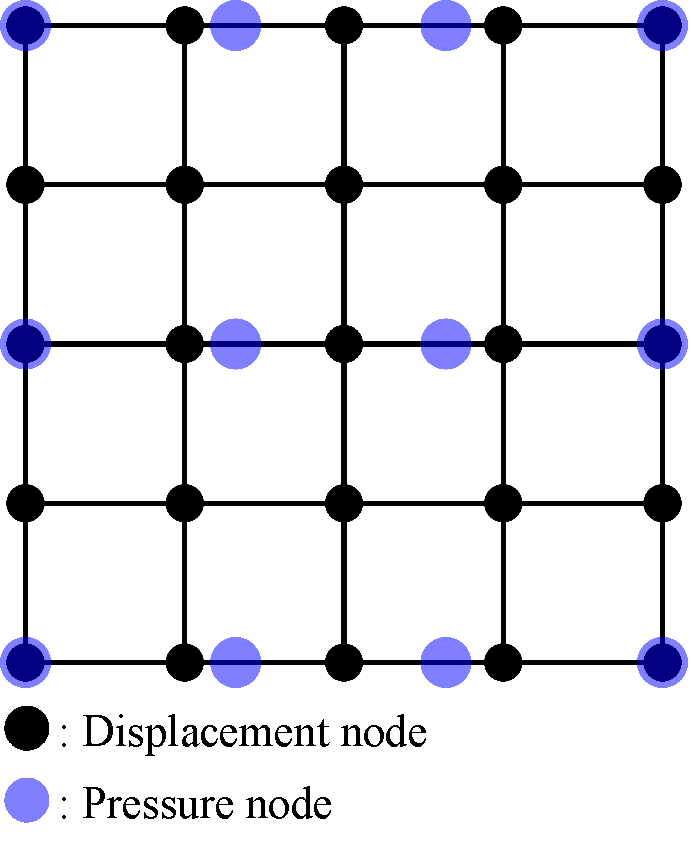
\includegraphics[width=0.5\textwidth]{pdf/infsup_mesh.pdf}
\caption{Illustration of uniform nodal distribution for inf--sup test with $n_u=5\times5$, $n_p=4\times3$}\label{fg:infsup_mesh}
\end{figure}

Figures \ref{fg:infsup_convergence_2D_a}--\ref{fg:infsup_convergence_3D_b} show the corresponding results, in which the red line stands for the value of $\beta$ with respect to the number of pressure nodes $n_p$, and the vertical dashed line denotes the stabilized number $n_s$. The deeper color of the lines means mesh refinement. The results show that, no matter linear or quadratic elements, as $n_p$ increases over $n_s$, the value of $\beta$ sharply decreases, and then the inf-sup condition cannot be maintained. This result is consistent with the discussion in Section \ref{sec:constraint_ratio}, and again verifies the effect of the proposed estimator.

Moreover, the mixed formulation's results with the traditional optimal constraint ratio $r=n_d$ are listed in these figures as well, and $\beta$ in this circumstance is already much smaller than those in the optimal range. Considering the results shown above, the easy programming and efficiency, the pressure nodes are chosen among the displacement nodes.
The optimal schemes for linear and quadratic, 2D and 3D element discretizations, namely with $r=r_{opt}$, are shown in Figure \ref{fg:mix_scheme},
where every other displacement node is selected as the pressure node.
For practical implementations of linear cases, the pressure nodes are initially generated using traditional approaches, such as Delaunay triangulation.
Subsequently, the displacement nodes are then obtained through a standard mesh refinement process to the pressure nodes.
For quadratic approximations in Tri6 and Quad8 elements, the element vertices are chosen as pressure nodes after displacement element generation.
Consequently, all constraint ratios evaluated using the discretizations in Figure \ref{fg:mix_scheme} fall within the optimal range.
The corresponding inf--sup test results for these schemes are also marked in inf--sup test figure and show that, with mesh refinement, their $\beta$'s are always maintained at a non-negligible level.

\begin{figure}[H]
\centering
\includegraphics[width=\textwidth]{png/tri3.png}
\caption{Inf--sup test for Tri3--RK}\label{fg:infsup_convergence_2D_a}
\end{figure}

\begin{figure}[H]
\centering
\includegraphics[width=\textwidth]{png/tri6.png}\caption{Inf--sup test for Tri6--RK}\label{fg:infsup_convergence_2D_b}
\end{figure}

\begin{figure}[H]
\centering
\includegraphics[width=\textwidth]{png/quad4.png}\caption{Inf--sup test for Quad4--RK}\label{fg:infsup_convergence_2D_c}
\end{figure}

\begin{figure}[H]
\centering
\includegraphics[width=\textwidth]{png/quad8.png}\caption{Inf--sup test for Quad8--RK}\label{fg:infsup_convergence_2D_d}
\end{figure}

\begin{figure}[H]
\centering
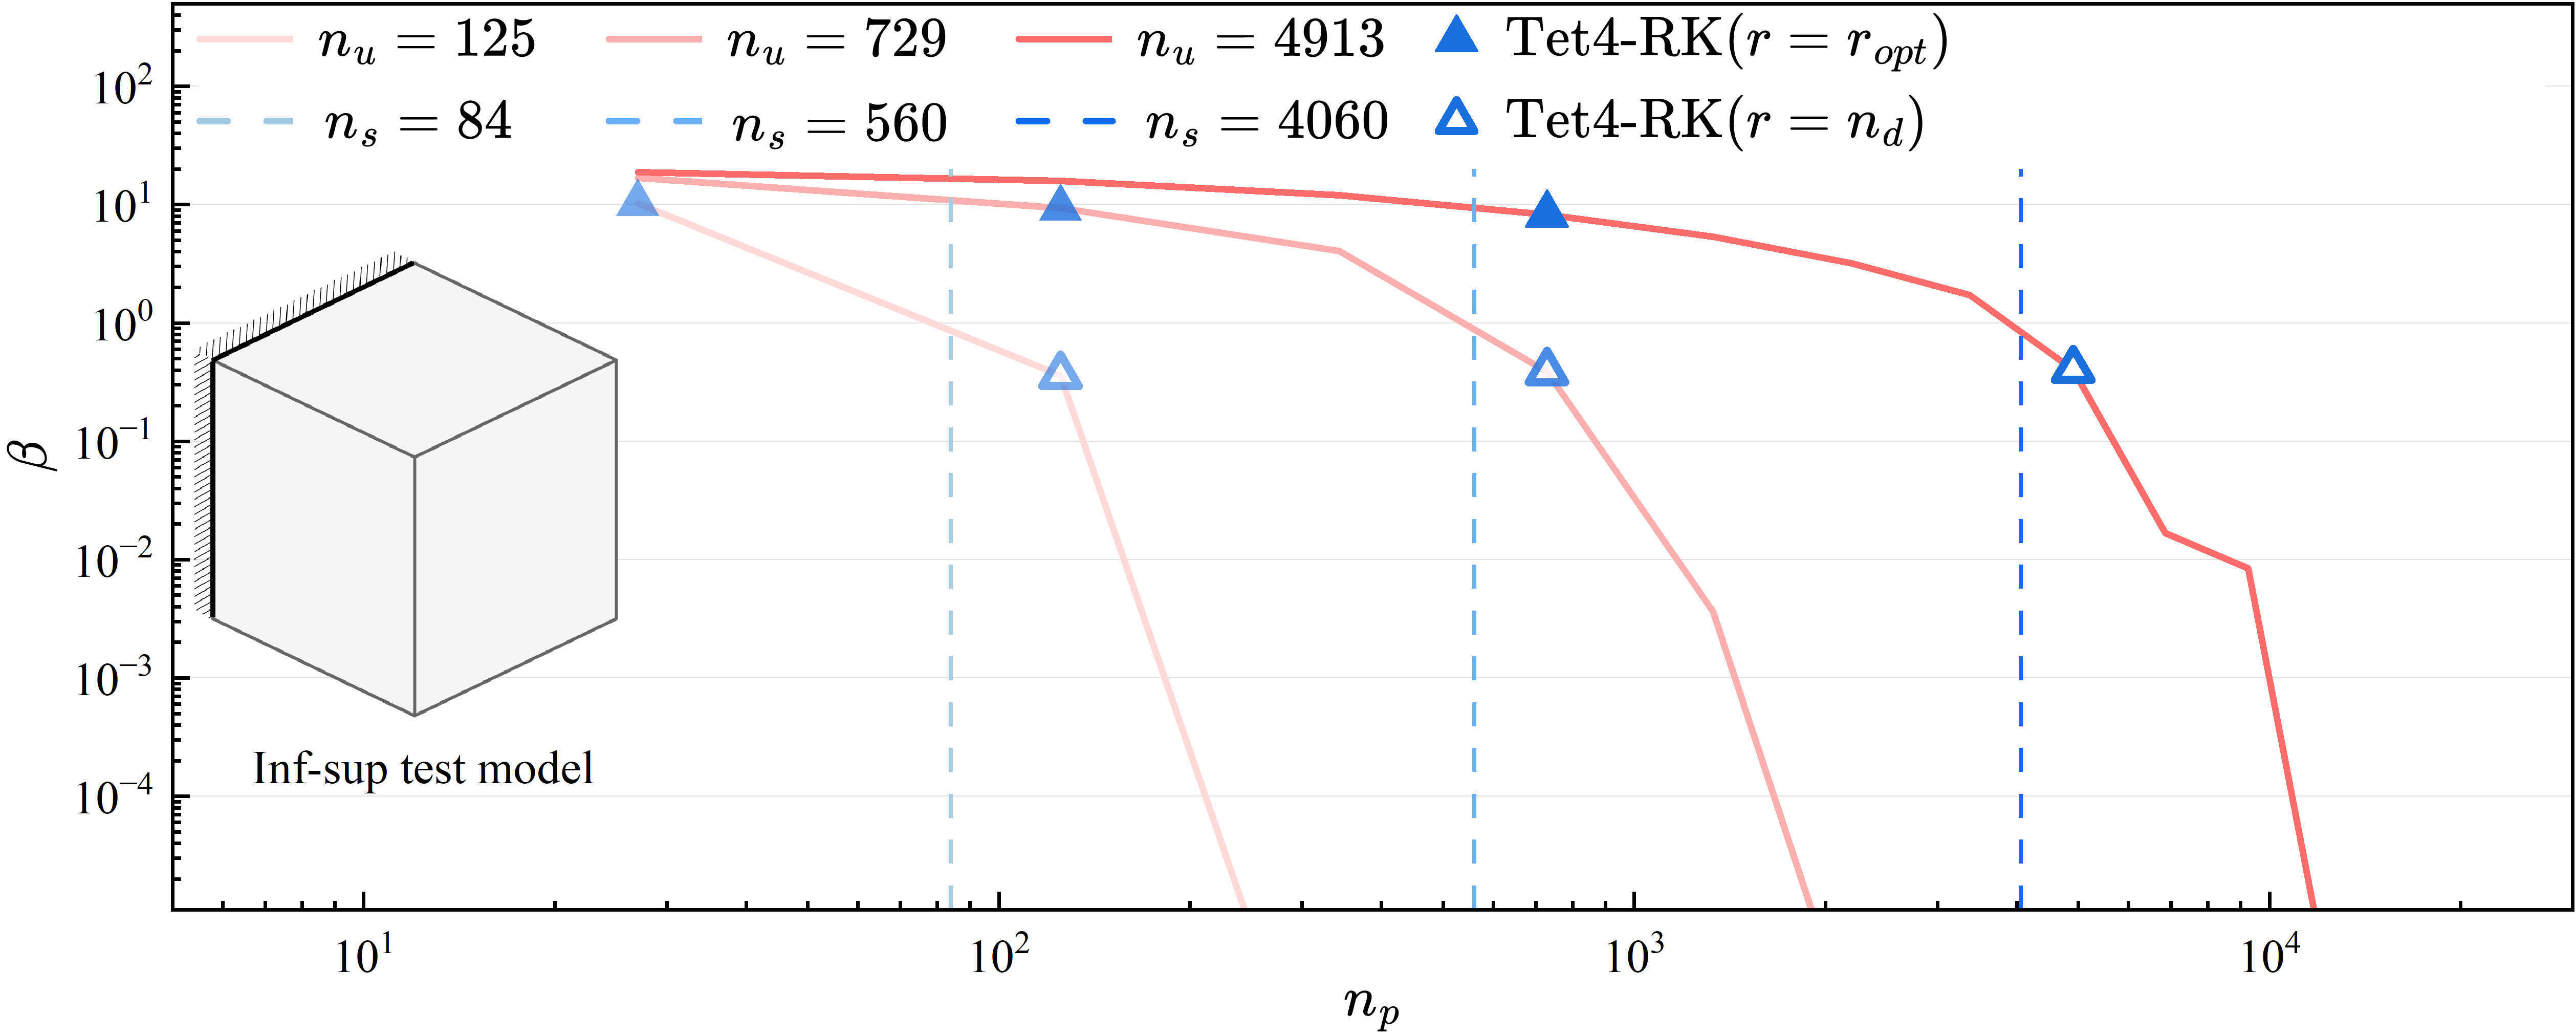
\includegraphics[width=\textwidth]{png/Tet4.png}\caption{Inf--sup test for Tet4--RK}\label{fg:infsup_convergence_3D_a}
\end{figure}

\begin{figure}[H]
\centering
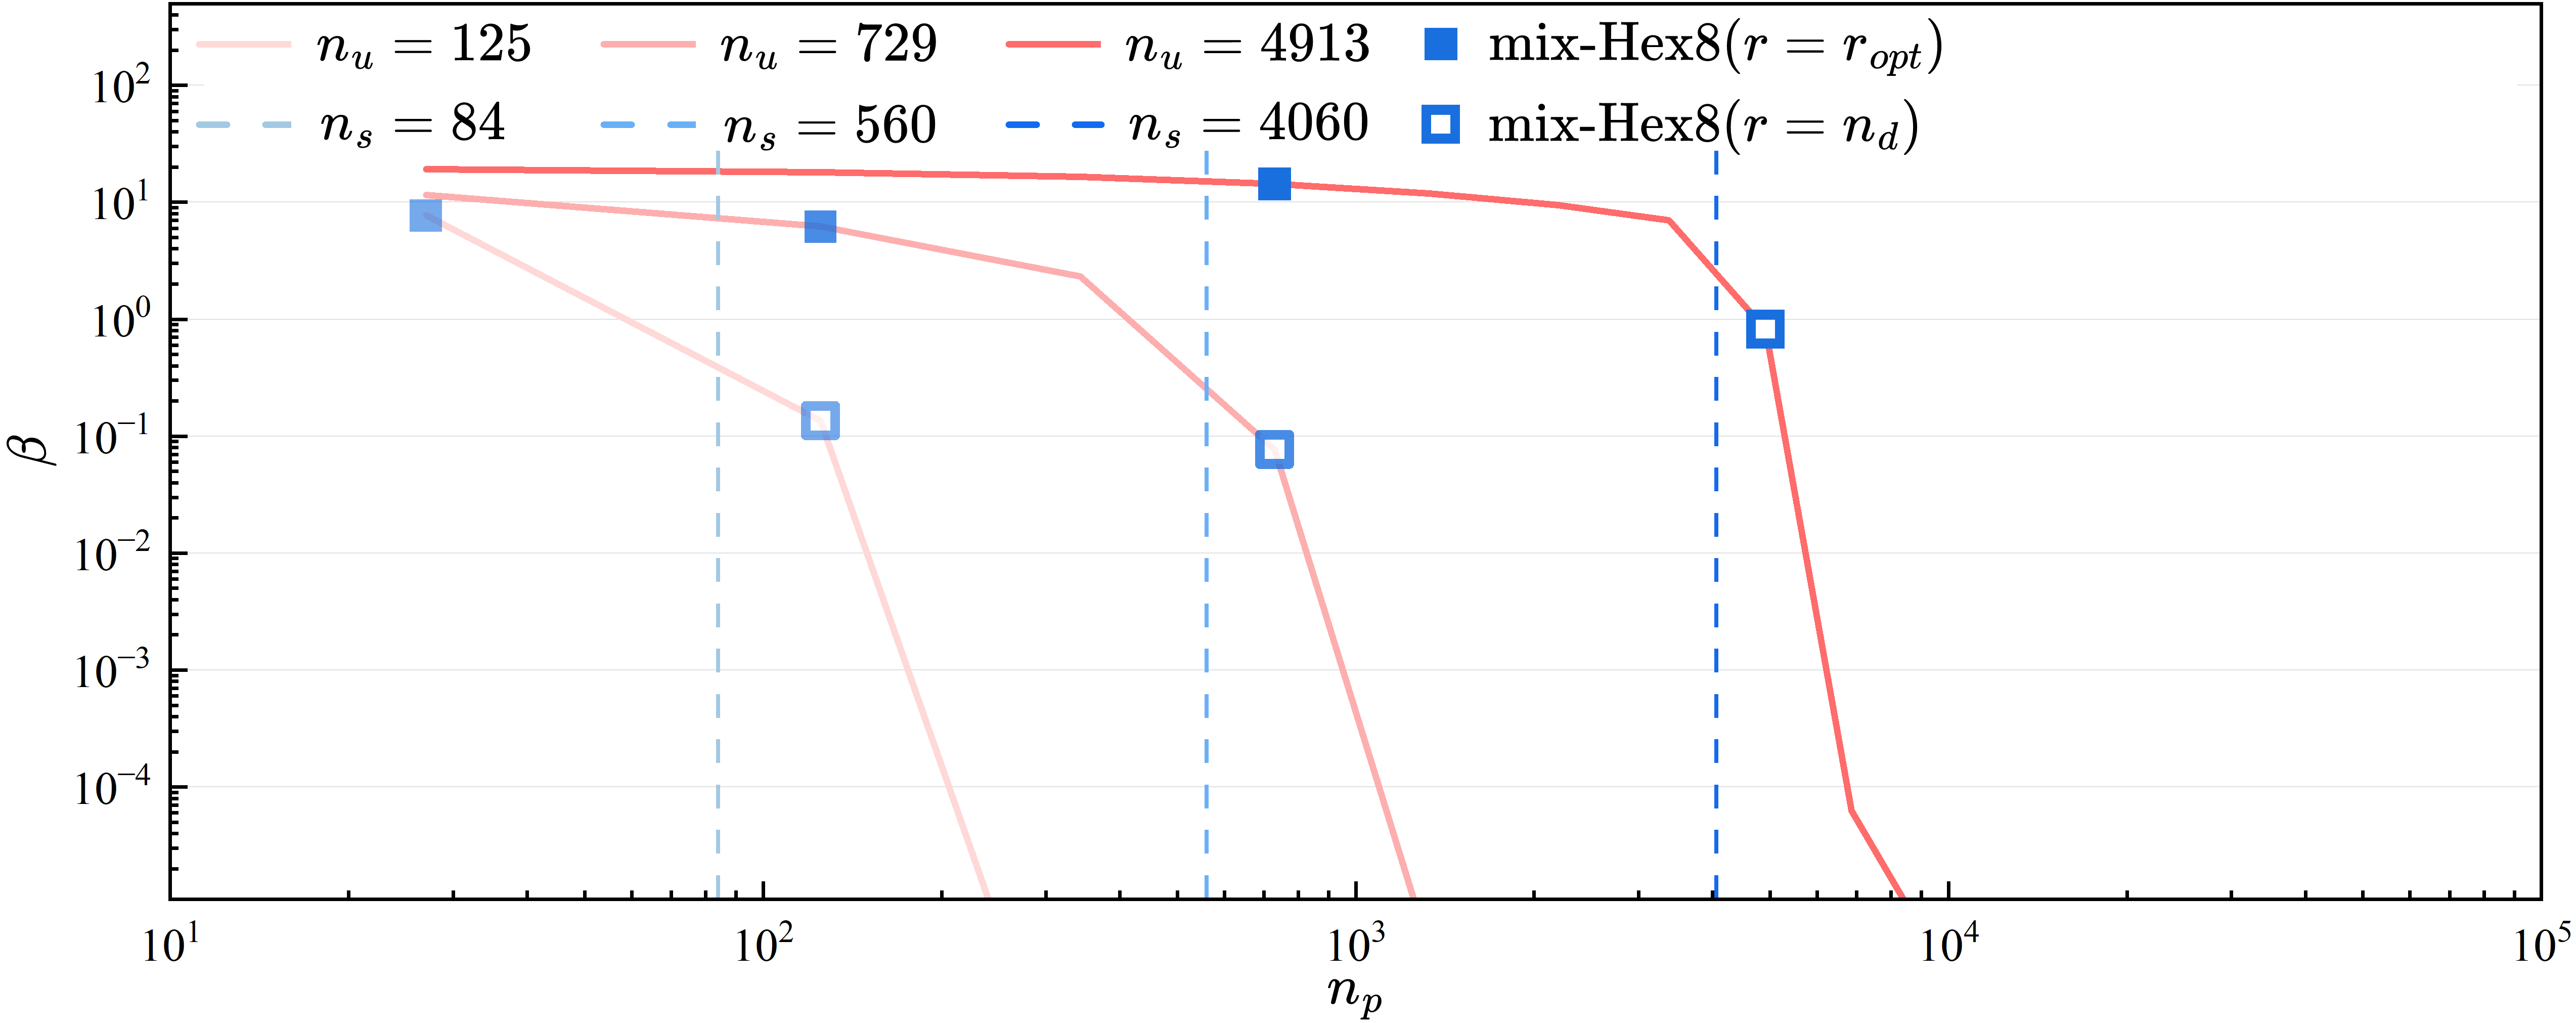
\includegraphics[width=\textwidth]{png/Hex8.png}\caption{Inf--sup test for Hex8--RK}\label{fg:infsup_convergence_3D_b}
\end{figure}

\begin{figure}[H]
\centering
\begin{tabular}{c@{\hspace{24pt}}c}
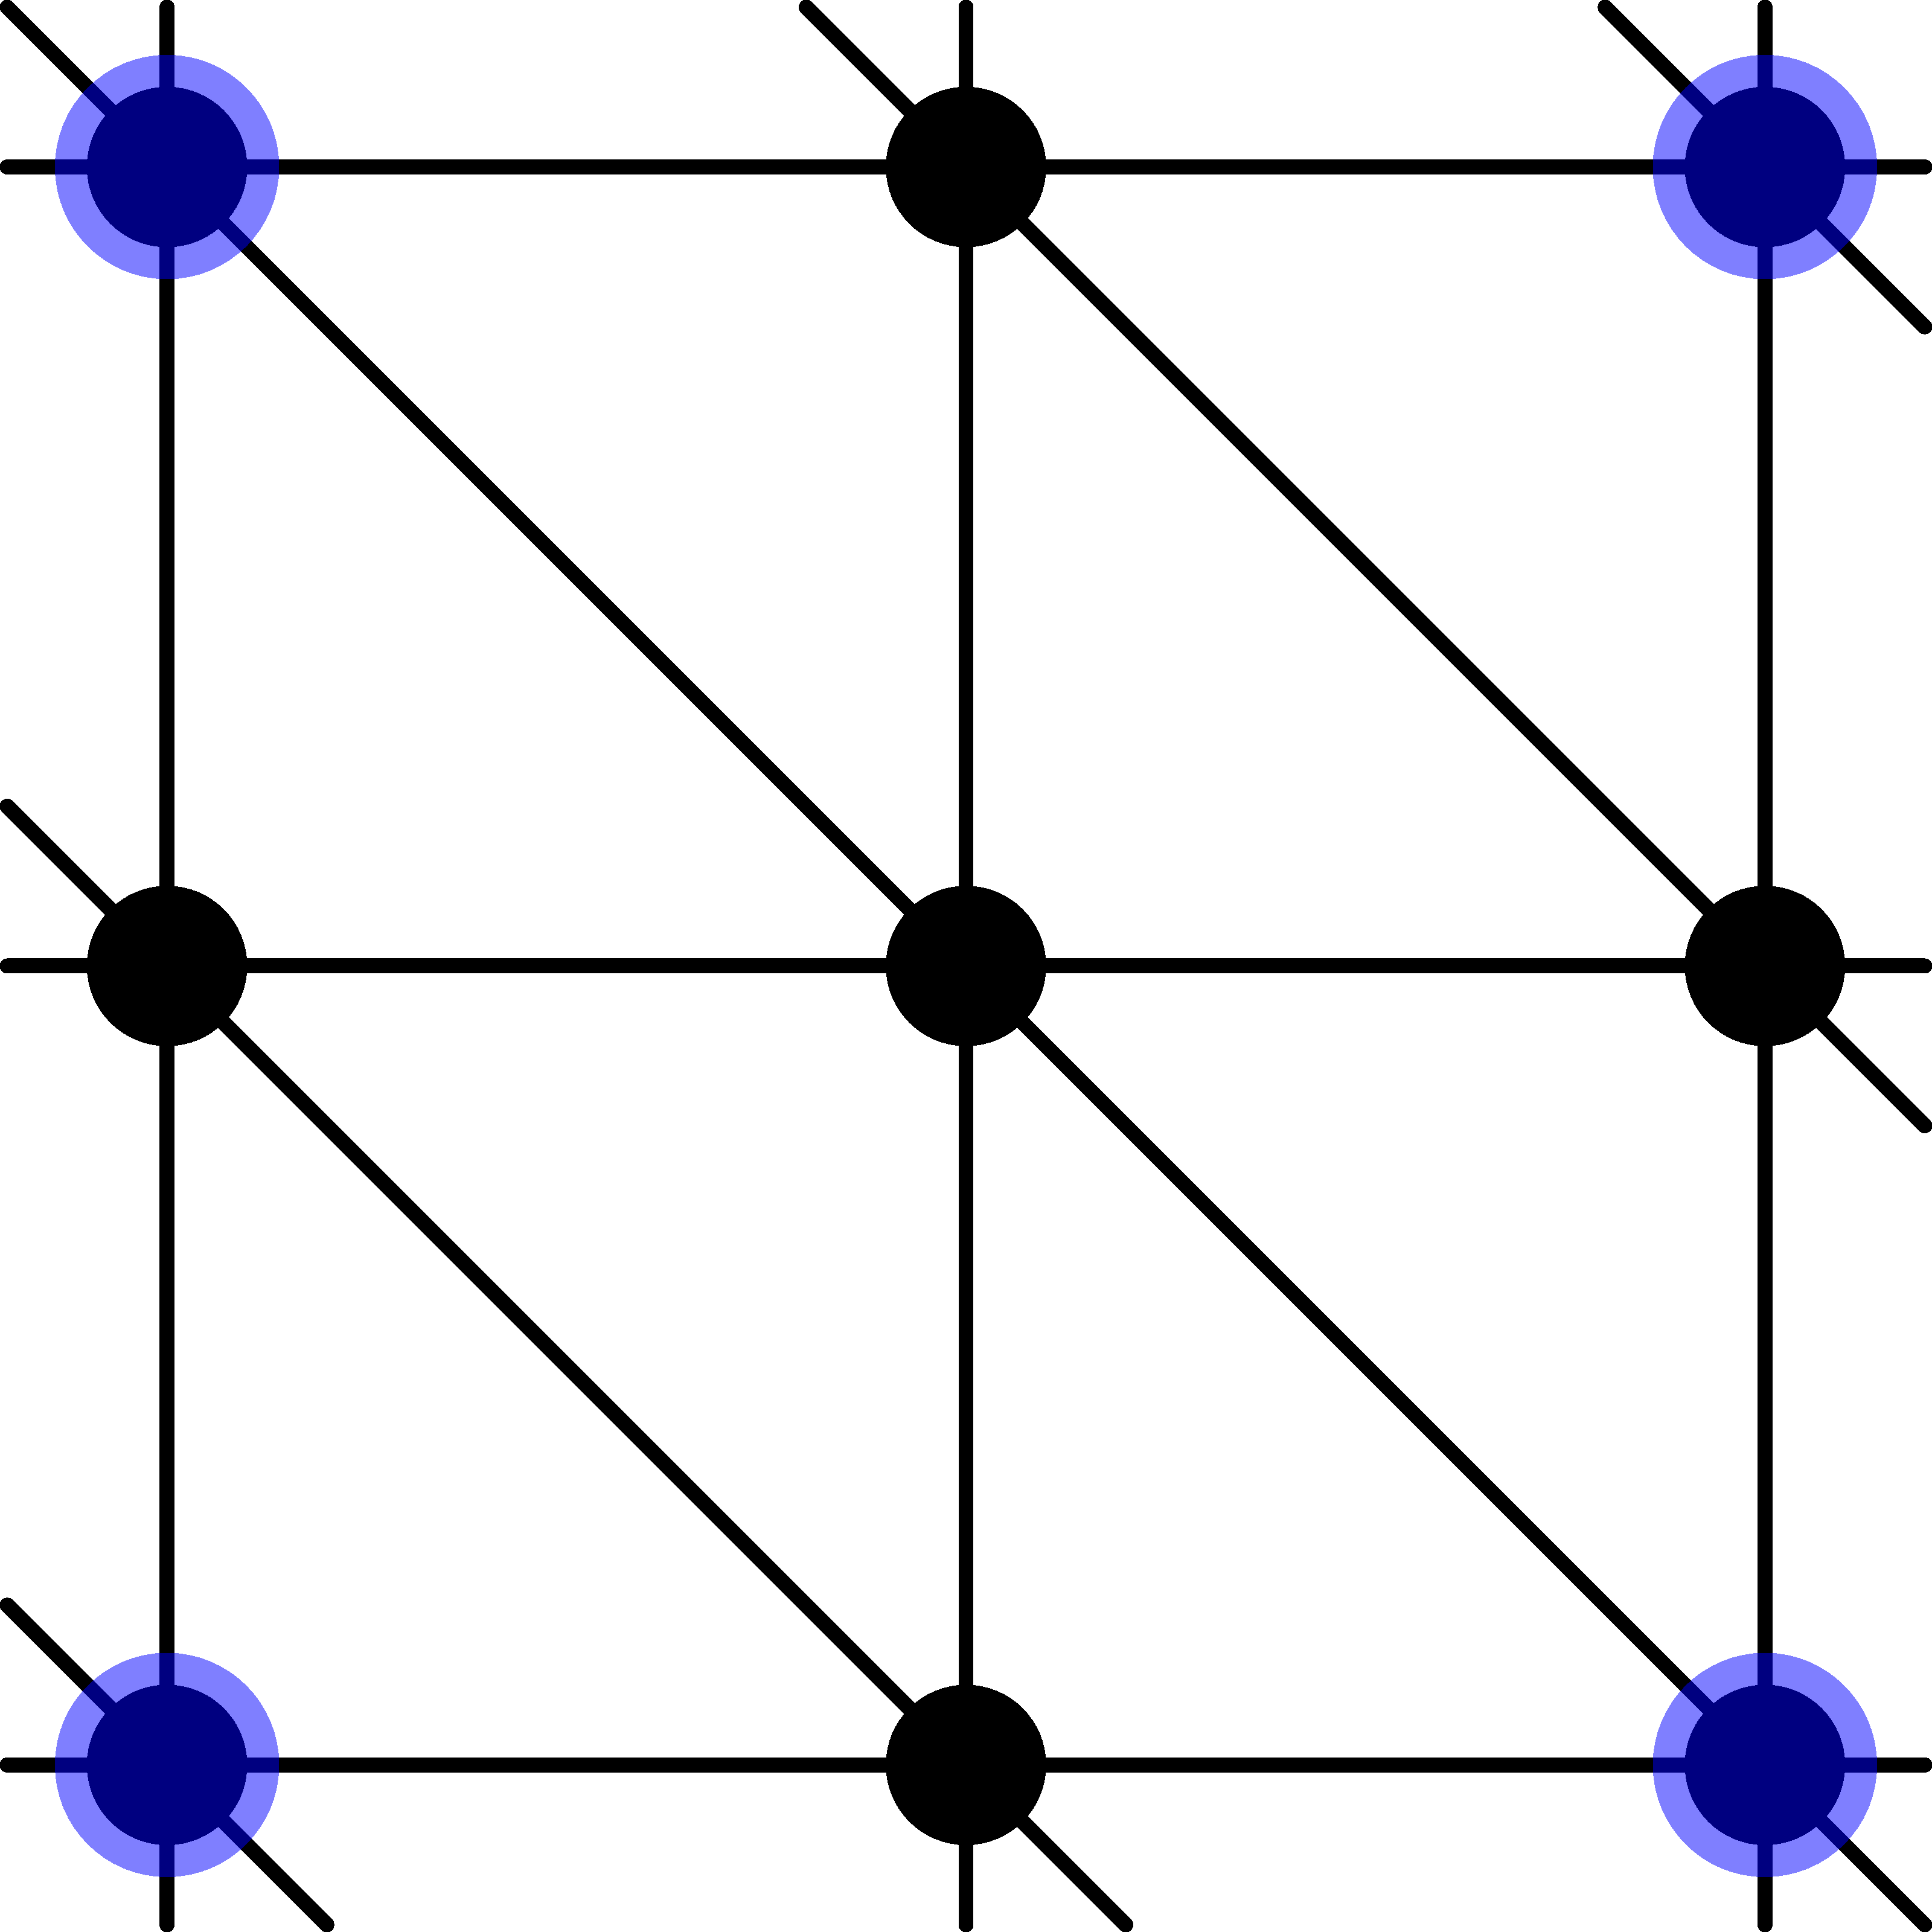
\includegraphics[width=0.28\textwidth]{png/mix_tri3.png} &
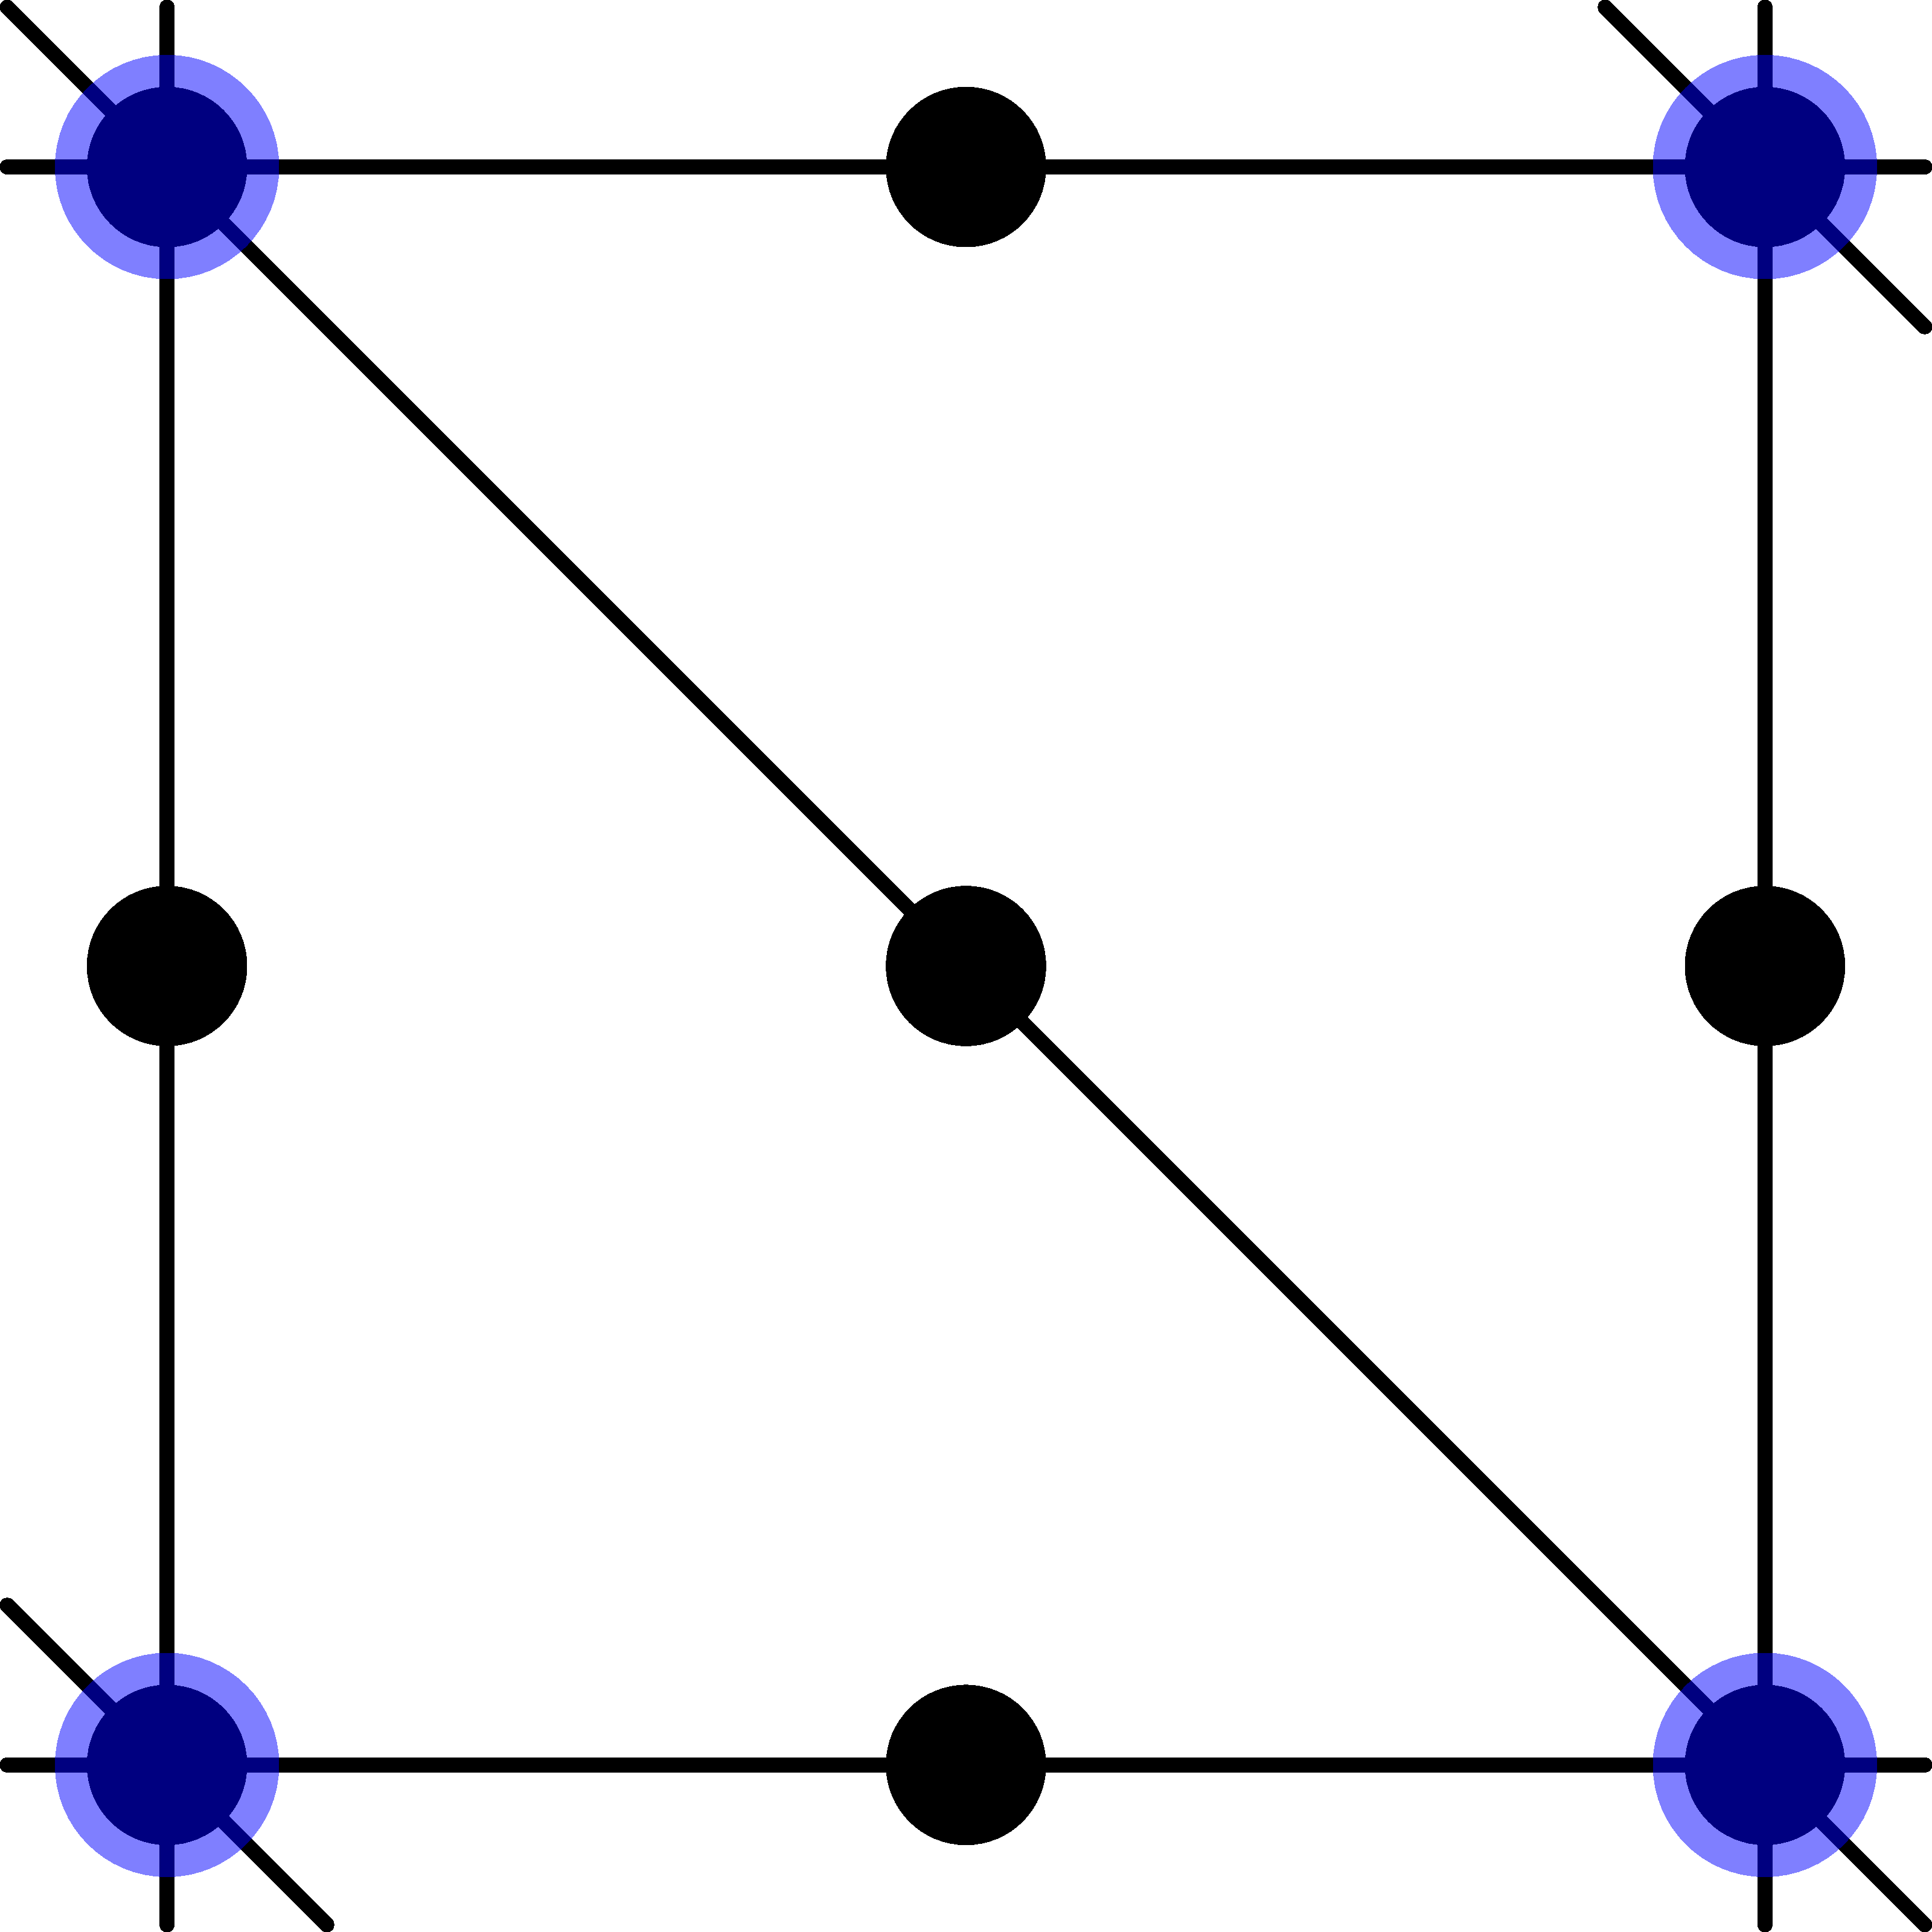
\includegraphics[width=0.28\textwidth]{png/mix_tri6.png} \\
Tri3--RK & Tri6--RK \\
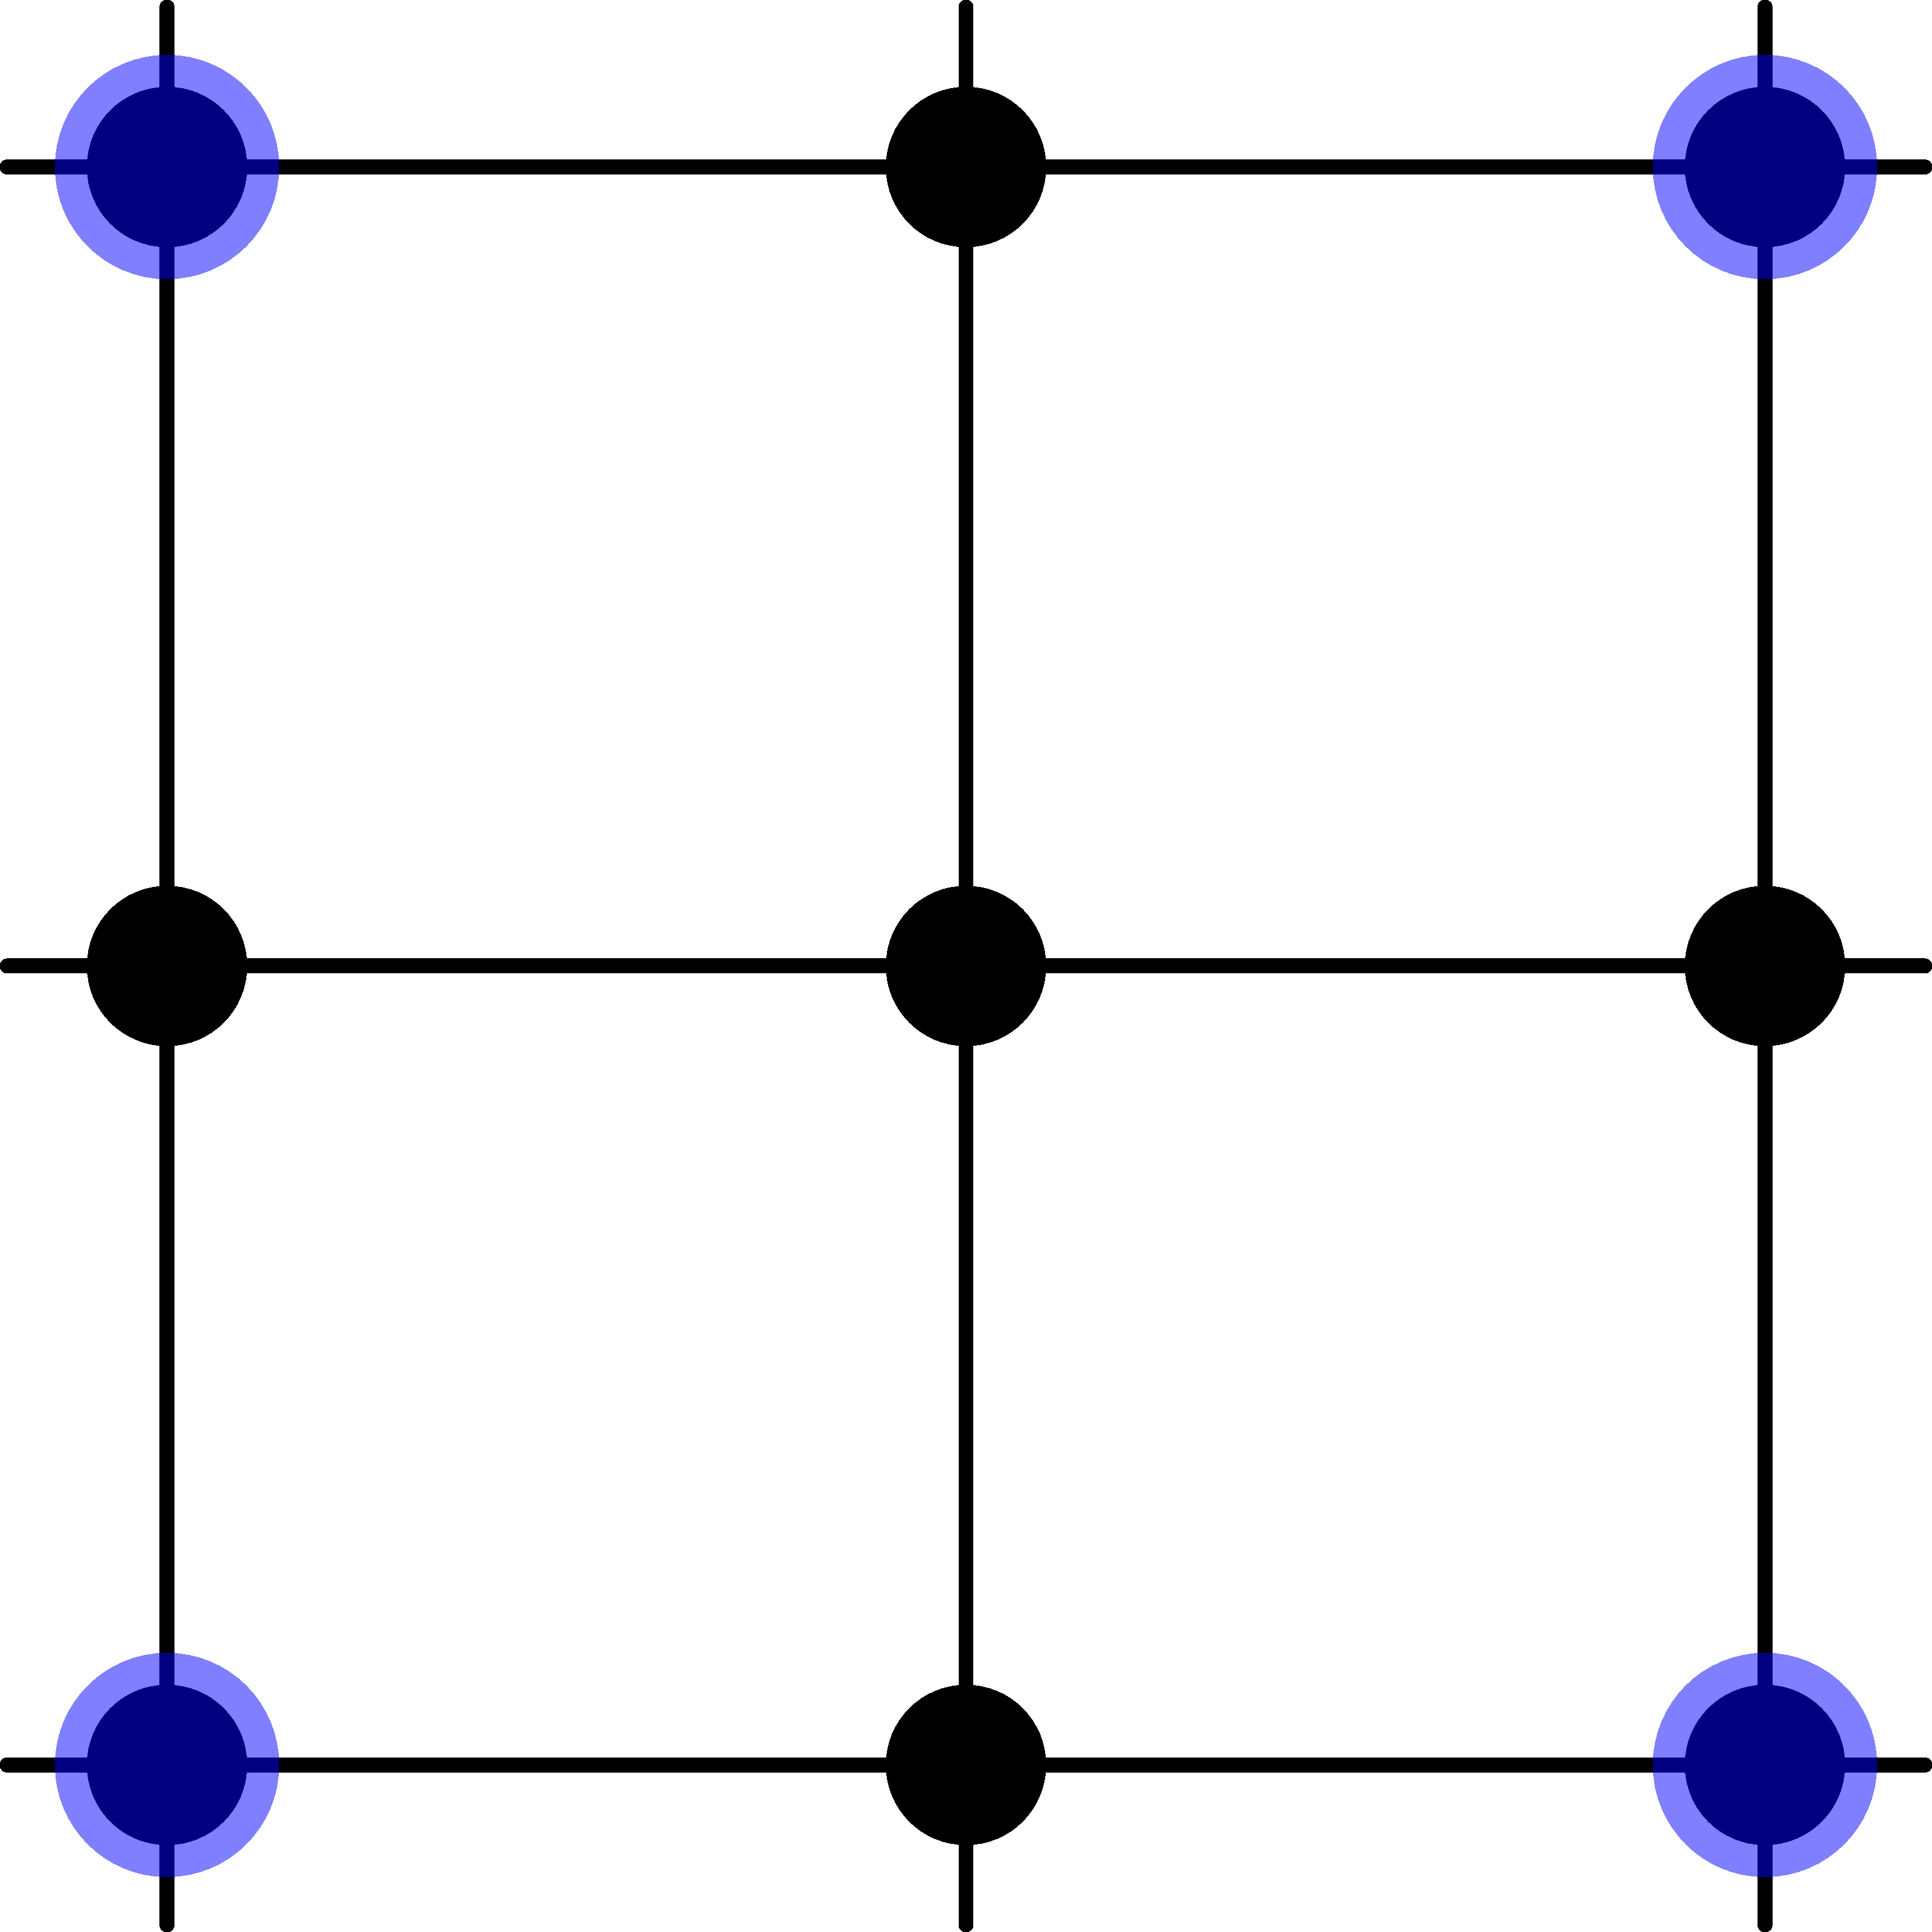
\includegraphics[width=0.28\textwidth]{png/mix_quad4.png} &
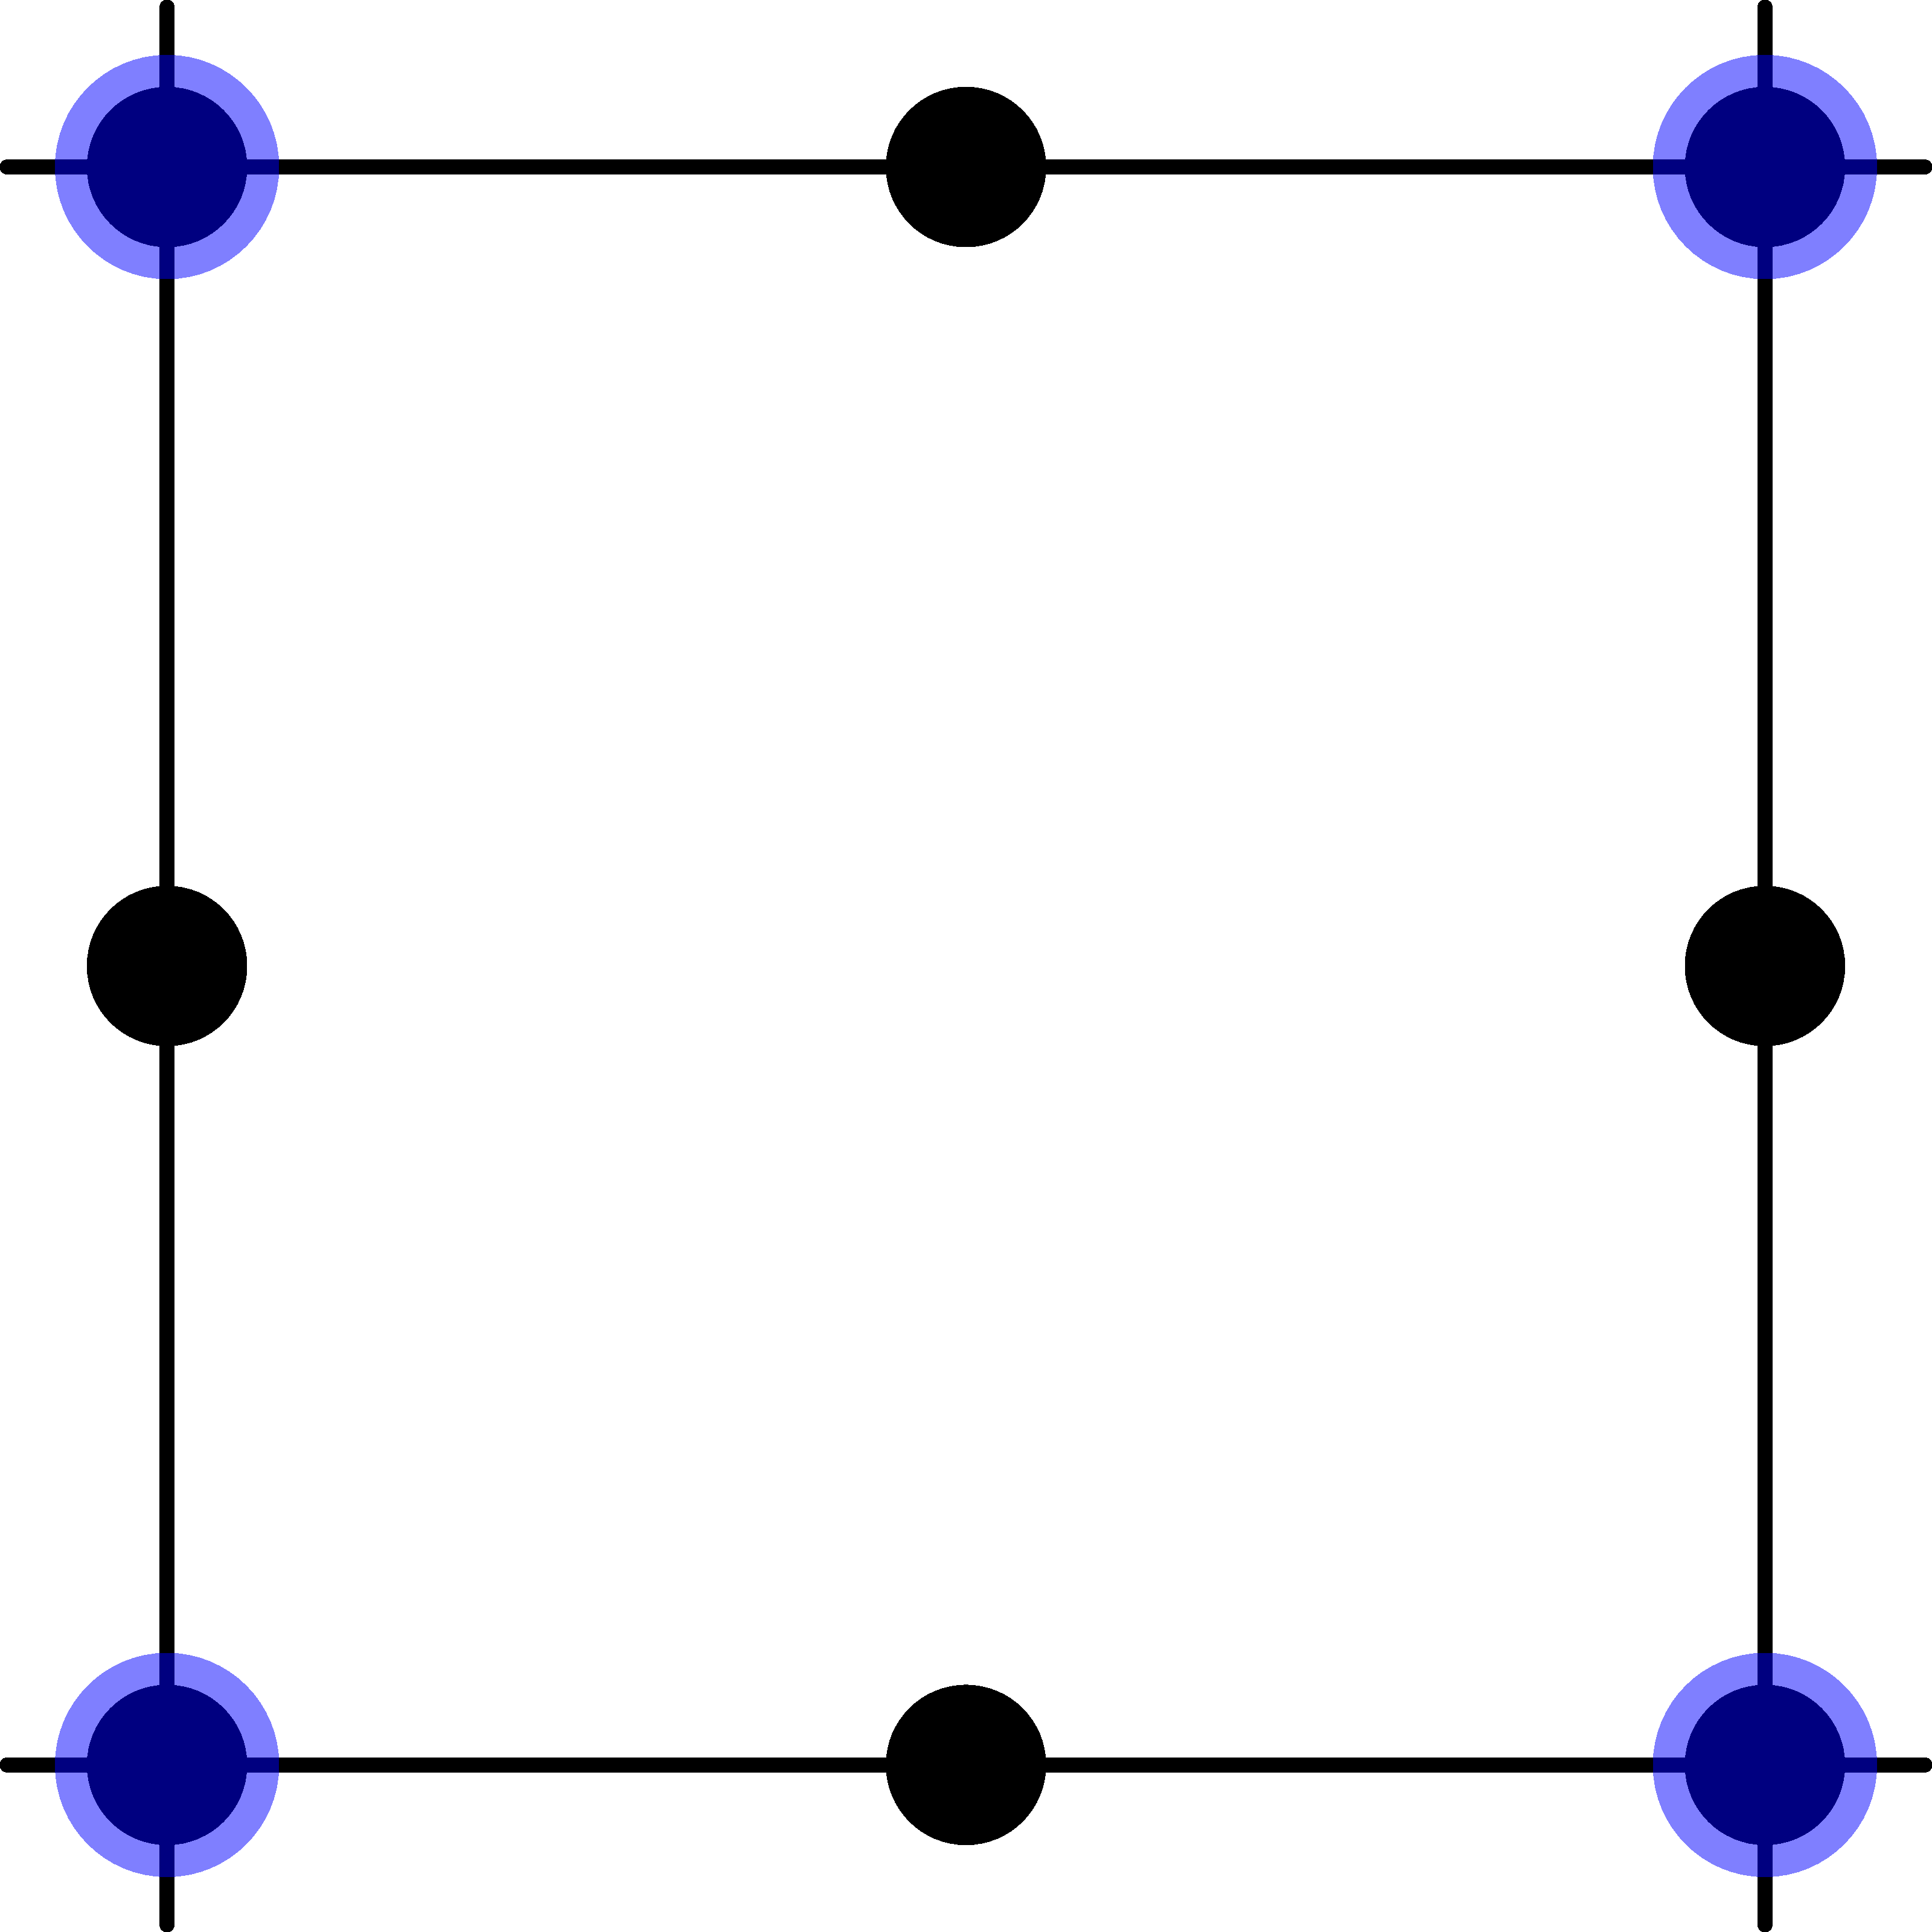
\includegraphics[width=0.28\textwidth]{png/mix_quad8.png} \\
Quad4--RK & Quad8--RK \\
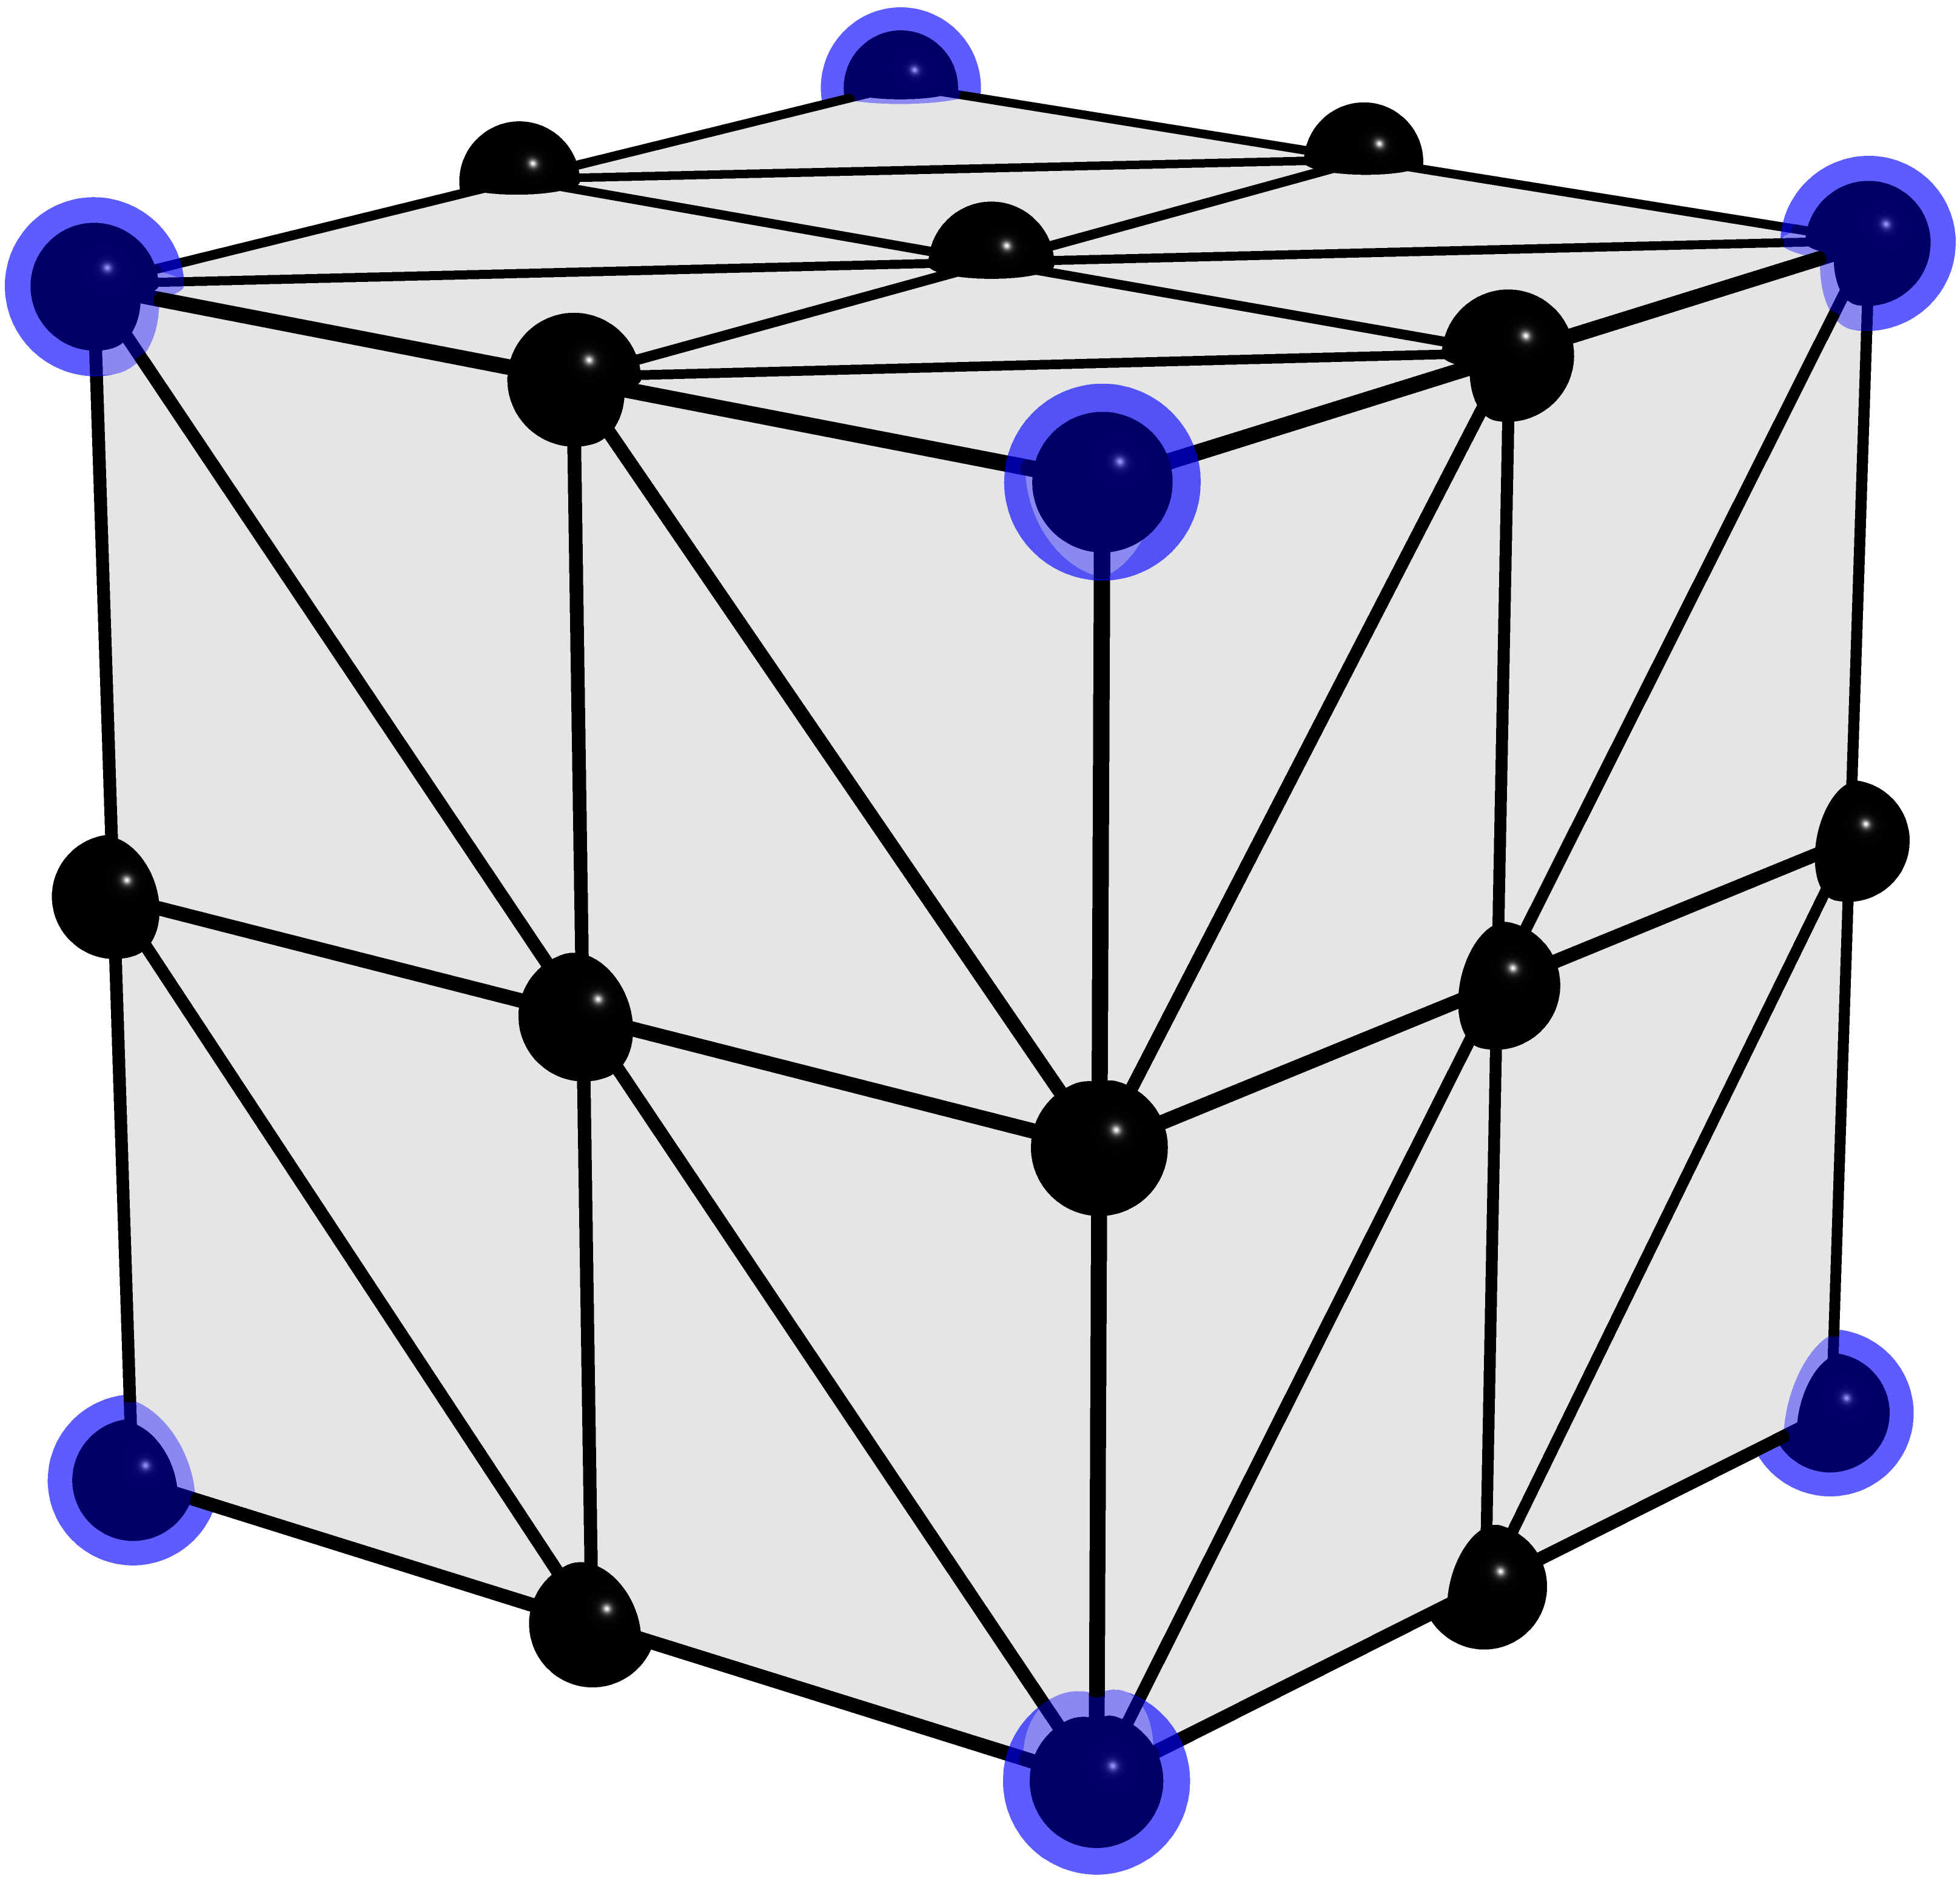
\includegraphics[width=0.28\textwidth]{png/mix_tet4.png} &
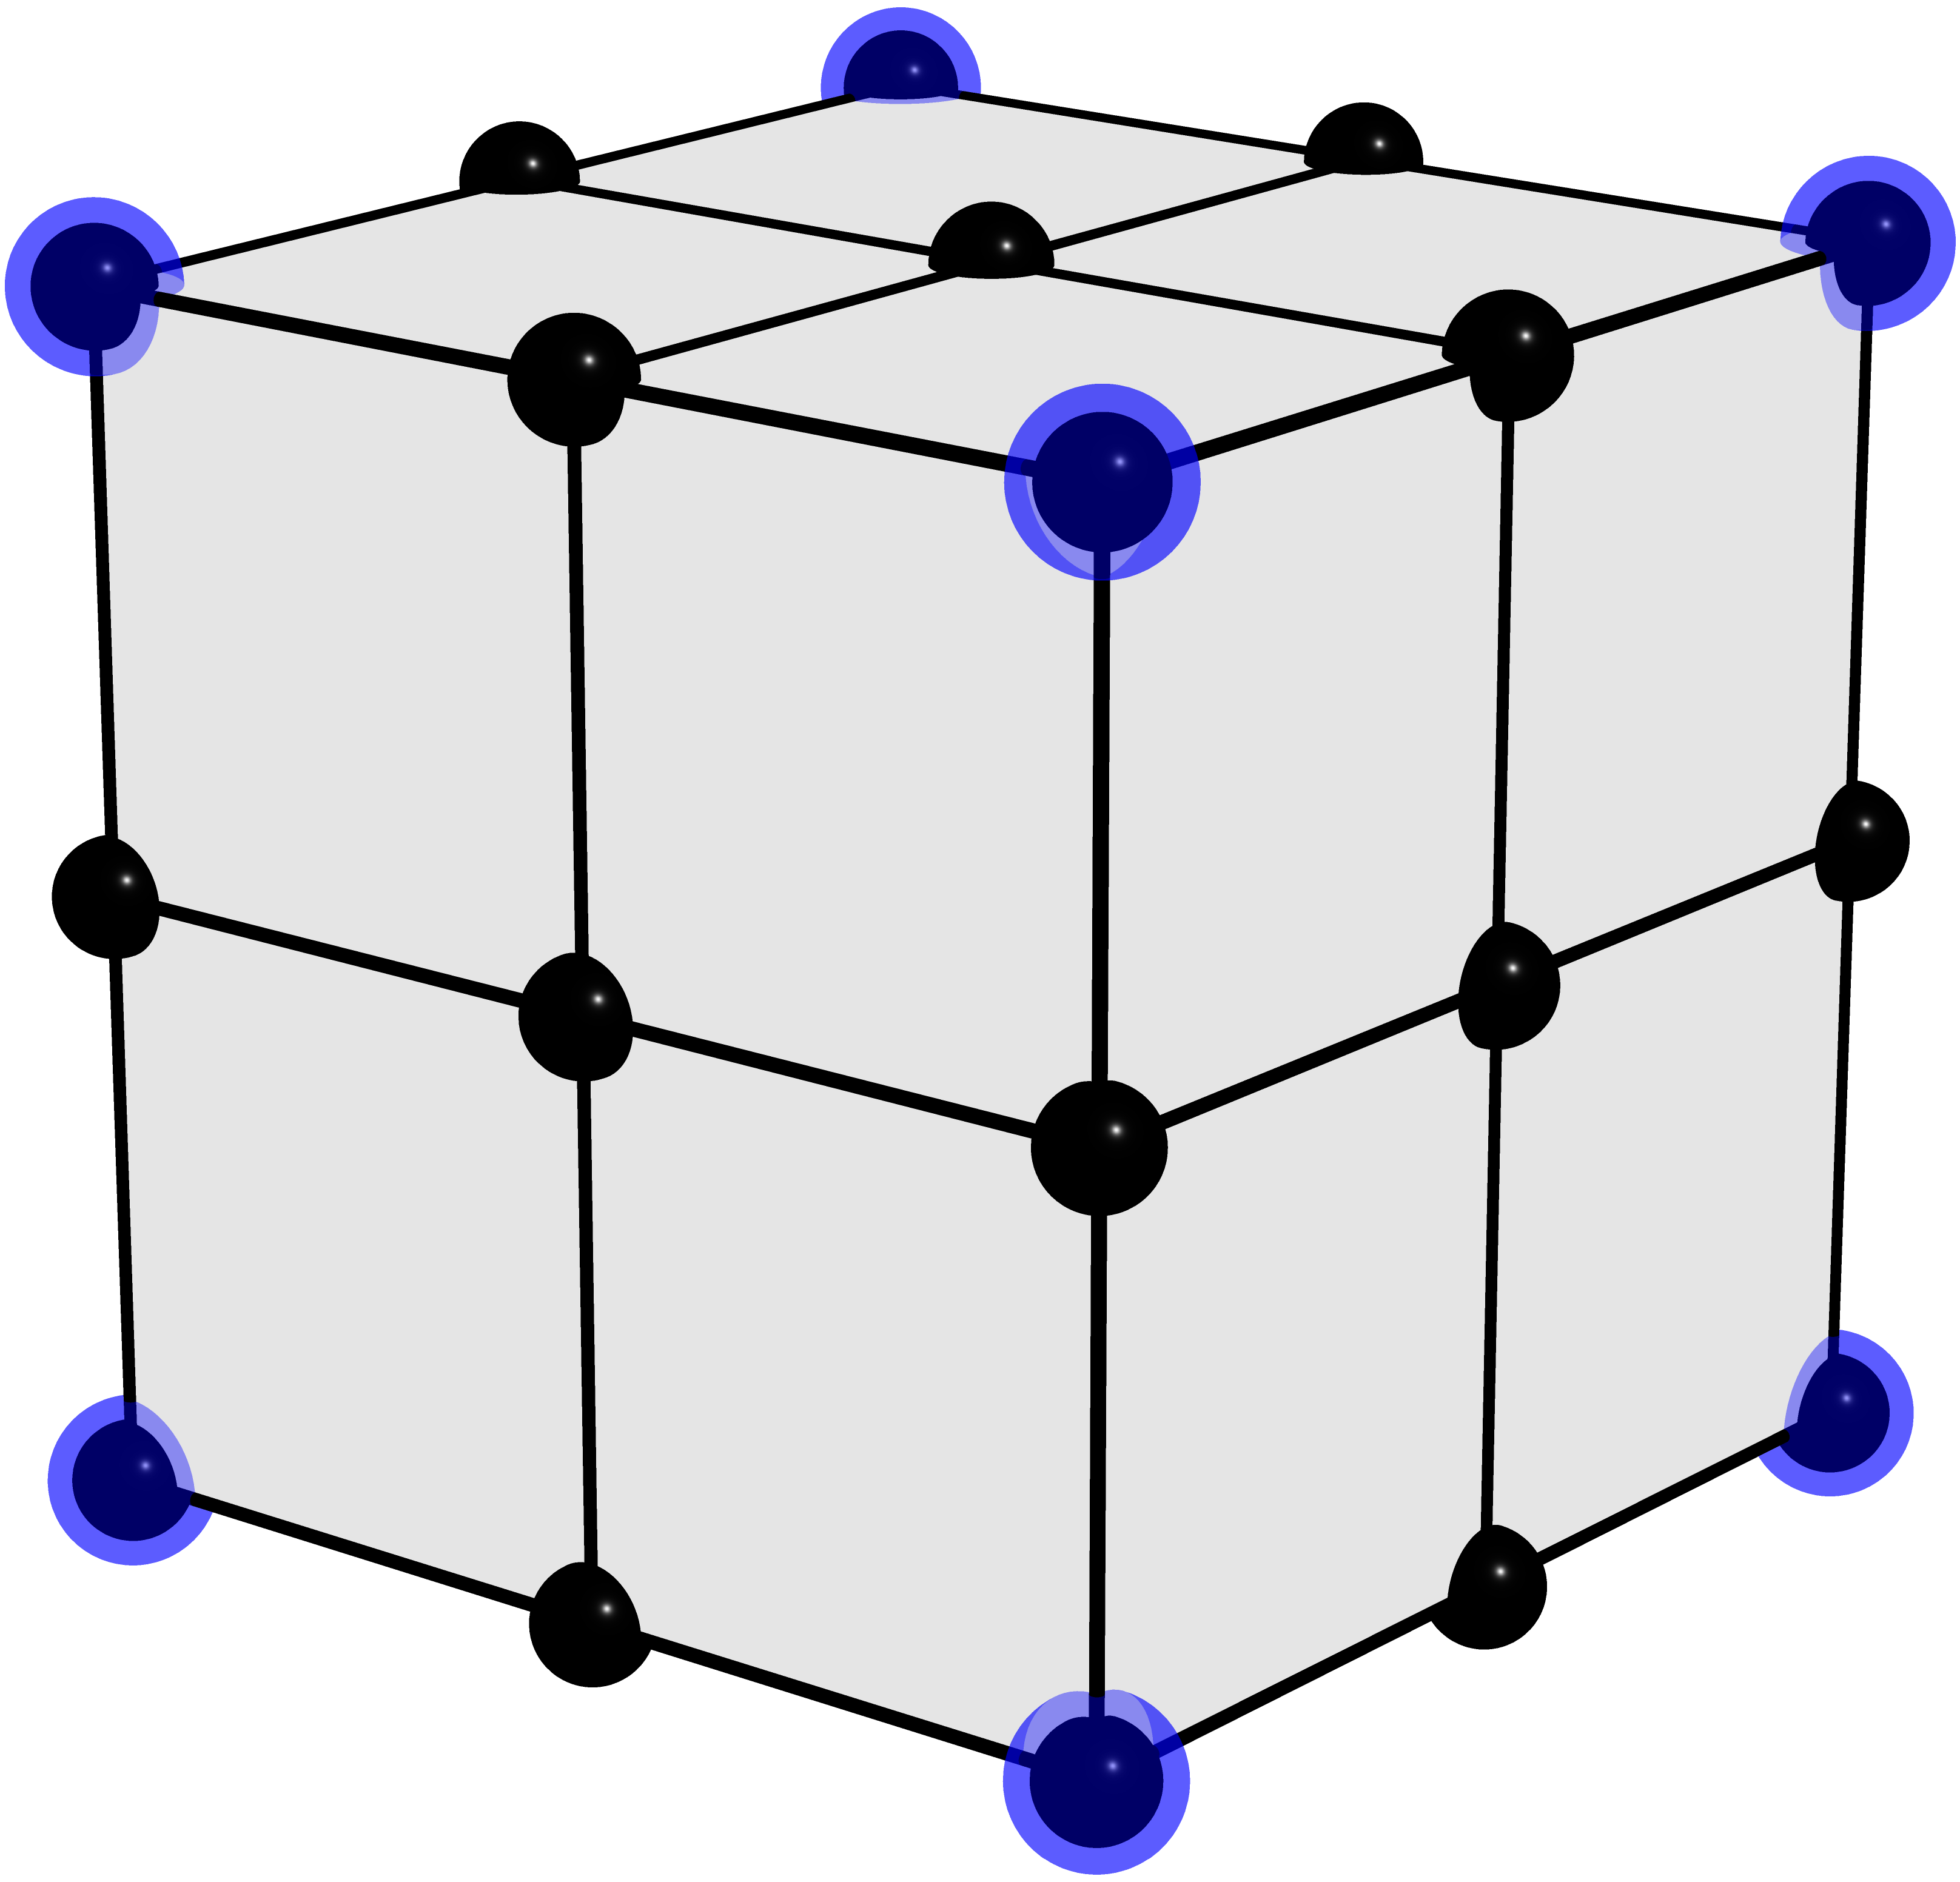
\includegraphics[width=0.28\textwidth]{png/mix_hex8.png} \\
Tet4--RK & Hex8--RK \\
\raisebox{-0.3\height}{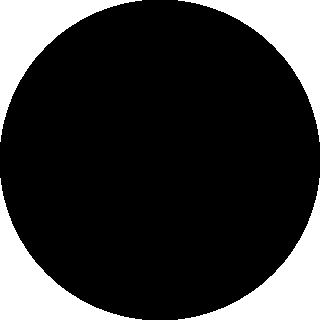
\includegraphics[width=12pt]{png/legend_u.png}} :Displacement node &
\raisebox{-0.3\height}{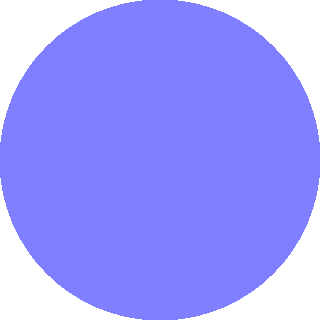
\includegraphics[width=12pt]{png/legend_p.png}} :Pressure node
\end{tabular}
\caption{Nodal distribution schemes for mixed FE-meshfree formulations with $r = r_{opt}$}\label{fg:mix_scheme}

\end{figure}

